\documentclass[11pt]{article}
\usepackage[utf8]{inputenc}
\usepackage{graphicx, mathtools, caption}
\usepackage{subcaption, listing}
\usepackage{amsmath, algorithm}
\usepackage[noend]{algpseudocode}

\topmargin -0.5in
\oddsidemargin -0.0in
\evensidemargin -0.0in
\textheight 9in
\textwidth 6.5in

\title{Python Implementation of Conway's Game of Life}
\author{Brad Green \& Edwin Weill}
\date{November 29, 2016}

\begin{document}
\maketitle

\section{Introduction}
The overall idea behind this project is to design a system that simulates \textit{Conway's Game of Life}, a cellular automaton.  Rather than being a "game" in which players interact with each other, this particular "game" is a zero-player game meaning that it goes through evolutions without any interaction with a player.  The only interaction the player has with the system is configuring the initial state and then lets the system evolve over time.
\par
The game is played on a two-dimensional grid of squares called \textit{cells}.  Each cell is categorized as either \textit{alive} or \textit{dead} at a particular "generation" of the simulation.  Each subsequent generation is determined by the interaction between neighbors (each cell interacts with its eight surrounding neighbors).  There are many rule variations that change the behavior of the system (i.e. how cells are spawned and how cells die).  The following set of rules is based on a rule variation known as B3/S23 (born with 3 neighbors, survive with 2 or 3 neighbors):
\begin{itemize}
	\item \textbf{Rule 1}: A living cell with fewer than 2 living neighbors dies (under-population)
	\item \textbf{Rule 2}: A living cell with 2 or 3 living neighbors lives to next generation
	\item \textbf{Rule 3}: A living cell with more than 3 living neighbors dies (over-population)
	\item \textbf{Rule 4}: A dead cell with 3 neighbors becomes alive (reproduction)
\end{itemize}

\section{Literature Review}

\section{Implementation}
The initial implementation simply uses the rules described above (or a similar rule strategy) to determine each generation in the evolution of the system and makes an updates based on each cell's neighbors.  The implementation iterates through every cell in the grid (alive or dead) and determines its next state based on the rules and neighbors.  The psuedocode in Algorithm \ref{naive_conway} illustrates this "naïve" algorithm implementation:
\begin{algorithm}
	\caption{Naïve Implementation Conway's Game of Life}\label{naive_conway}
	\begin{algorithmic}[1]
		\Procedure{Naive Conway}{$width, height, cell\_initialization, max\_iterations$}
			\State $grid\gets initialize\_grid(cell\_initialization)$
			\State $count\gets 0$
			\While{$count < max\_iterations$}\Comment{Update until limit reached}
				\If{$no\ change\ from\ previous\ generation$}
					\State exit
				\EndIf
				\State $count\gets count+1$
				\For{$y < grid\_height$}
					\For{$x < grid\_width$}
						\If{$cell\ is\ living$}
							\If{$cell\ has\ 2\ or\ 3\ neighbors$}
								\State $cell.state\gets dead$
							\EndIf
						\Else
							\If{$cell\ has\ 3\ neighbors$}
								\State $cell.state\gets alive$
							\EndIf
						\EndIf
					\EndFor
				\EndFor
			\EndWhile\label{naiveendwhile}
		\EndProcedure
	\end{algorithmic}
\end{algorithm}

\section{Optimizations}
The above implementation is rather simplistic and therefore it does not perform well for larger board sizes.  The naive implementation is of computational order O(width*height) which means that every cell must be visited during each evolution between generations.  This is highly inefficient when the board size gets large, therefore slowing down its execution.  For this reason, optimizations need to be employed utilizing various data structures to alleviate the need to "visit" every cell in the grid.
\subsection*{Set of Living Cells}
The first optimization technique makes use of an additional set which holds all cells which are currently living.  The strategy only checks for modifications in cells that are currently living and all neighbors of the living cells.  For each cell, we keep a count of how many cells it touches, which can be used to check the rules and add cells to the new \textit{living} list.  This implementation is much more efficient as the number of rule checks is significantly decreased for most instances of a typical grid layout, O(number of living cells).
\subsection*{Quadtree}
ADD PARAGRAPH ABOUT QUADTREE HERE

\section{Results}
\subsection{Visualization Results}
There are many different patterns that the game of life lends itself to when started in certain configurations.  For example, there are some patterns which do not change not matter how long the simulation is run (unless they are interacted with by another living cell).  There are others that oscillate between a set number of states; these patterns are called oscillators.  Figure \ref{fig:still} illustrates a \textit{box} which is an example of a still pattern while Figure \ref{fig:oscillator} illustrates a pattern with a period (an oscillator).
\begin{figure}[!ht]
	\centering
	\begin{subfigure}{.45\textwidth}
		\centering
  	  	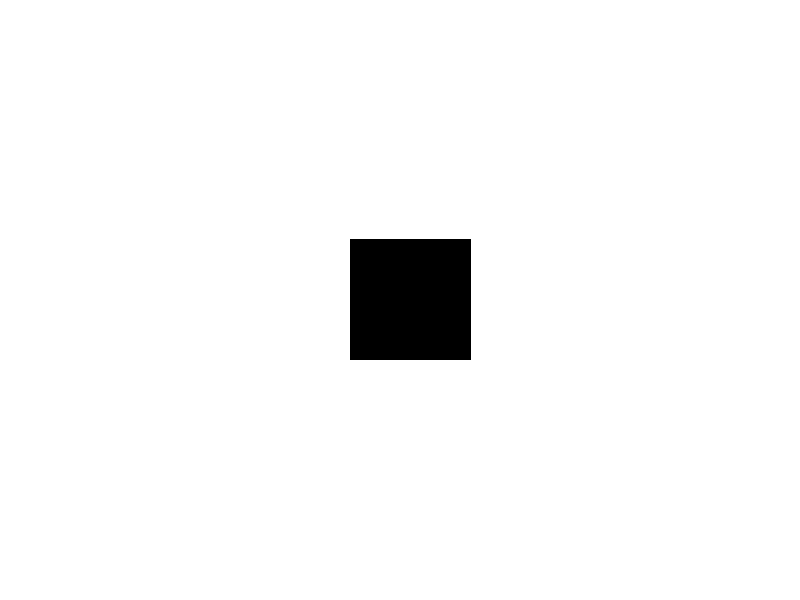
\includegraphics[width=1\linewidth]{images/box.png}
  	  	\label{fig:box1}
	\end{subfigure}
	\begin{subfigure}{.45\textwidth}
  	  	\centering
  	  	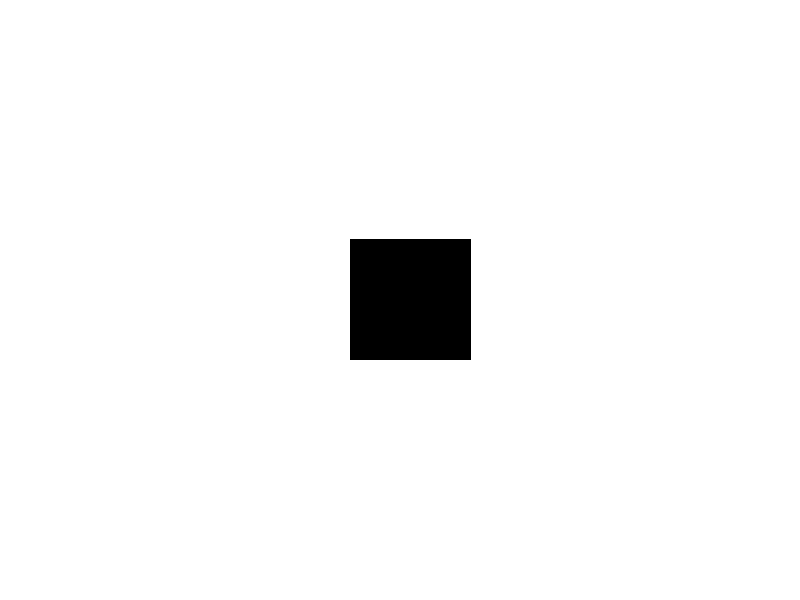
\includegraphics[width=1\linewidth]{images/box.png}
  	  	\label{fig:box2}
	\end{subfigure}
	\caption{Still Positions 1 \& 2}
	\label{fig:still}
\end{figure}

\begin{figure}[!ht]
	\centering
	\begin{subfigure}{.45\textwidth}
		\centering
  	  	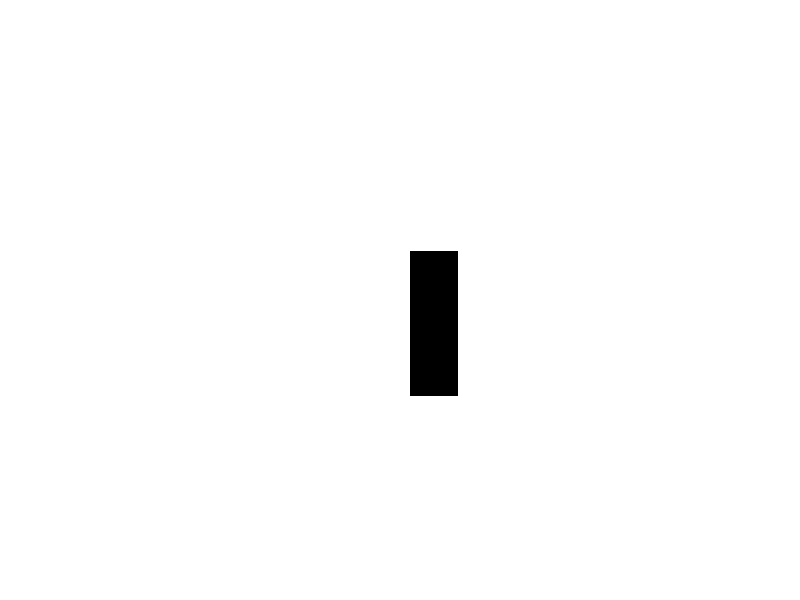
\includegraphics[width=1\linewidth]{images/blinker1.png}
  	  	\label{fig:blinker1}
	\end{subfigure}
	\begin{subfigure}{.45\textwidth}
  	  	\centering
  	  	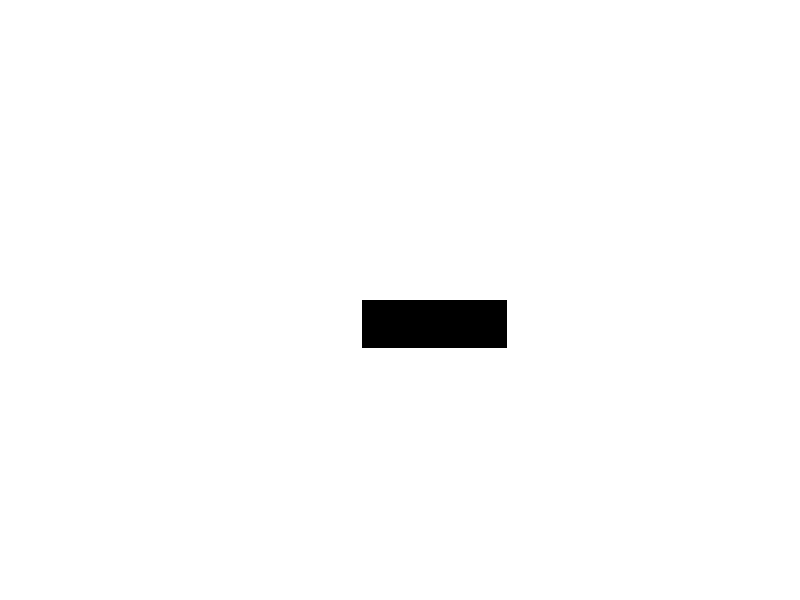
\includegraphics[width=1\linewidth]{images/blinker2.png}
  	  	\label{fig:blinker2}
	\end{subfigure}
	\caption{Oscillator Positions 1 \& 2}
	\label{fig:oscillator}
\end{figure}

There are many other types of patterns that facilitate good visualizations including glider guns (shown in Figure \ref{fig:glider_gun}).  The glider is created from the \textit{gun} every 30 iterations based on the B3/S23 rule strategy.  Another interesting example is a single live cell beginning the game with the automaton B1/S12 resulting in a very close approximation of the Sierpinski triangle.  Figure \ref{fig:sierpinski_triangle} illustrates this example.

\begin{figure}[!ht]
	\centering
	\begin{subfigure}{.45\textwidth}
		\centering
  	  	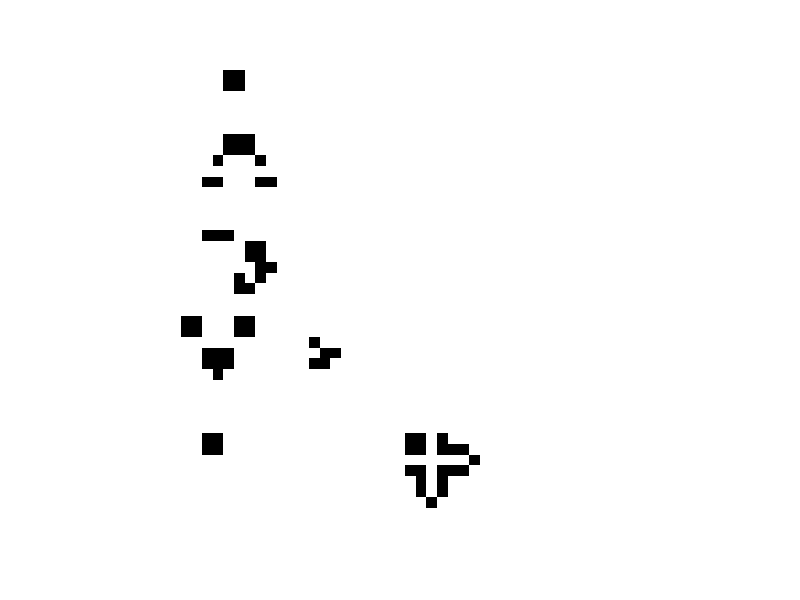
\includegraphics[width=1\linewidth]{images/glider_gun1.png}
  	  	\label{fig:glider_gun1}
	\end{subfigure}
	\begin{subfigure}{.45\textwidth}
  	  	\centering
  	  	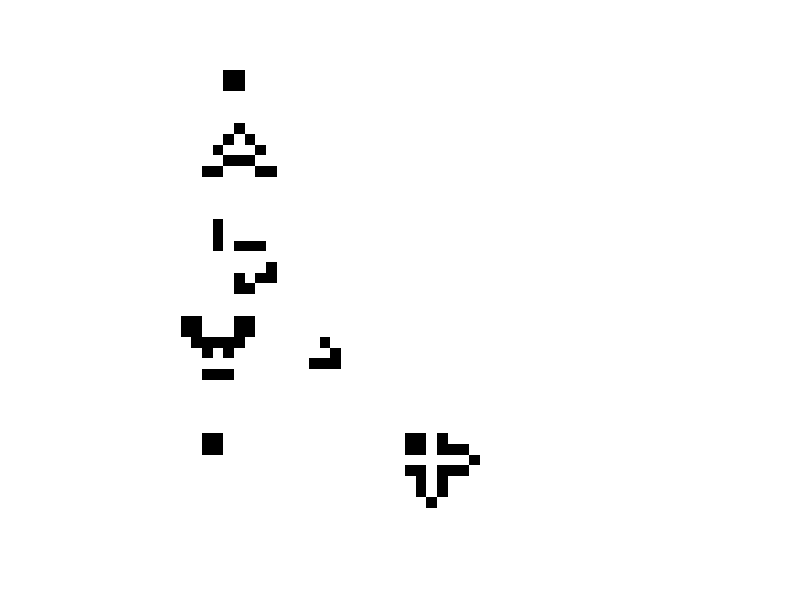
\includegraphics[width=1\linewidth]{images/glider_gun2.png}
  	  	\label{fig:glider_gun2}
	\end{subfigure}
	\caption{Glider Gun Positions 1 \& 2}
	\label{fig:glider_gun}
\end{figure}

\begin{figure}[!ht]
	\centering
	\begin{subfigure}{\textwidth}
		\centering
  	  	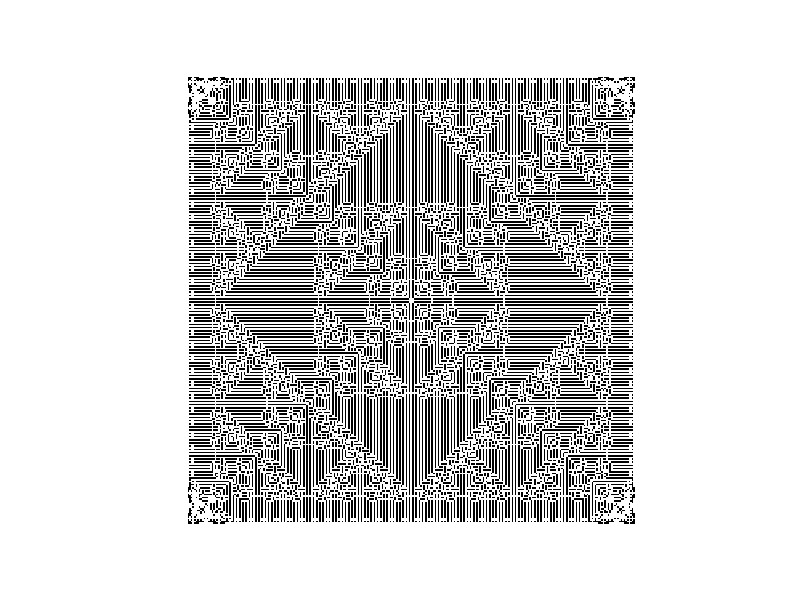
\includegraphics[width=1\linewidth]{images/sierpinski.png}
  	  	\label{fig:sierpinski1}
	\end{subfigure}
	\caption{Sierpinski Triangle}
	\label{fig:sierpinski_triangle}
\end{figure}

\subsection{Performance Results}

\section{Discussion}

\section{Distribution of Work}


\end{document}